\documentclass[conference]{IEEEtran}
\IEEEoverridecommandlockouts

% ---------------------- PREÁMBULO ----------------------
\usepackage{cite}
\usepackage{tikz}
\usetikzlibrary{calc,positioning,arrows.meta}
\usepackage[ruled,vlined,linesnumbered]{algorithm2e}
\usepackage{listings}
\usepackage[most]{tcolorbox} % opcional, pero recomendado
\usepackage{amsmath,amssymb,amsfonts}
\usepackage{mathtools}
\usepackage{algorithmic}
\usepackage{graphicx}
\usepackage{textcomp}
\usepackage{threeparttable}
\usepackage{xcolor}
\usepackage{float}
\usepackage{tabularx} % tablas adaptables al ancho
\usepackage{booktabs} % reglas bonitas en tablas
\usepackage{siunitx}  % alineación numérica
\usepackage{caption}
\usetikzlibrary{arrows.meta,positioning,decorations.pathreplacing,matrix}
\usepackage{placeins}   % para \FloatBarrier
\usepackage{graphicx}
\usepackage{enumitem}
\usetikzlibrary{arrows.meta,positioning,decorations.pathreplacing}
\usepackage{tabularx}
\newcolumntype{L}{>{\raggedright\arraybackslash}X}
\usepackage{needspace}   % reservar espacio antes de un bloque grande
\allowdisplaybreaks[0]   % NO partir ecuaciones multi-línea entre páginas
\interdisplaylinepenalty=10000


\setlength{\jot}{6pt}        % Más espacio vertical entre líneas en align

% --- AJUSTES PARA EVITAR SOLAPES ---
\usepackage{microtype}     % mejor espaciado y cortes
\usepackage[bottom]{footmisc}
\usepackage{stfloats}      % mejor colocación de floats
\usepackage{dblfloatfix}   % floats a dos columnas fiables
\usepackage{balance}
\usepackage{etoolbox}
\appto\sloppy{}            % más permisivo con los cortes
\emergencystretch=3em      % evita overfull hboxes
\allowdisplaybreaks[2]     % permite partir ecuaciones si hace falta
\raggedbottom              % evita estirar vertical en exceso

% --- Código en una sola página y sin desbordes ---
\usepackage{listings}
\usepackage{courier}
\lstset{
  basicstyle=\footnotesize\ttfamily,
  breaklines=true,
  breakatwhitespace=true,
  frame=single,
  columns=fullflexible,
  keepspaces=true,
  showstringspaces=false,
  tabsize=2
}

\sisetup{table-number-alignment=center,round-mode=places,round-precision=2}
\renewcommand{\arraystretch}{1.2} % más aire entre filas
\captionsetup{font=small,labelfont=bf}
\setlength{\abovecaptionskip}{4pt}
\setlength{\belowcaptionskip}{4pt}
\setlength{\textfloatsep}{8pt plus 2pt minus 2pt}
\setlength{\floatsep}{8pt plus 2pt minus 2pt}
\setlength{\intextsep}{6pt plus 2pt minus 2pt}
\graphicspath{{./}}

\def\BibTeX{{\rm B\kern-.05em{\sc i\kern-.025em b}\kern-.08em
    T\kern-.1667em\lower.7ex\hbox{E}\kern-.125emX}}

% ---------------------- DOCUMENTO ----------------------

\title{Heuristic Approaches for the $k$-Traveling Salesman Problem: A Reproducible Comparison\thanks{}}

\author{\IEEEauthorblockN{1\textsuperscript{st} Nicolás Barrientos}
\IEEEauthorblockA{\textit{Facultad de Ingeniería} \\
\textit{Universidad Andrés Bello}\\
Santiago de Chile, Chile \\
n.barrientossabaleta@uandresbello.edu}
\and
\IEEEauthorblockN{2\textsuperscript{nd} Gustavo Gatica}
\IEEEauthorblockA{\textit{Facultad de Ingeniería} \\
\textit{Universidad Andrés Bello}\\
Santiago de Chile, Chile \\
ggatica@unab.cl}
\and
\IEEEauthorblockN{3\textsuperscript{rd} Daniel Morillo-Torres}
\IEEEauthorblockA{\textit{Facultad de Ingeniería} \\
\textit{Pontificia Universidad Javeriana Cali}\\
Cali, Colombia \\
daniel.morillo@javerianacali.edu.co}
\and
\IEEEauthorblockN{4\textsuperscript{th} Rodrigo Linfati}
\IEEEauthorblockA{\textit{Departamento de Ingeniería Industrial} \\
\textit{Universidad del Bío-Bío}\\
Concepción, Chile \\
rlinfati@ubiobio.cl}
}
\begin{document}

\maketitle

\begin{abstract}
The $k$-Traveling Salesman Problem ($k$-TSP) is a variation of the classical Traveling Salesman Problem (TSP). Given a set of $n$ cities that includes a home city (depot) and a fixed value $k$ with $1 < k \le n$, the $k$-TSP seeks a single tour of minimum total length that starts and ends at the home city and visits \emph{exactly} $k$ cities (the home city included), chosen from the $n$ available. Solving it therefore involves two coupled decisions: \emph{which} $k$ cities to visit and in \emph{which order}.

This work presents a repository and an experimental implementation of several optimization techniques for the $k$-TSP, including a greedy cheapest-insertion constructive heuristic, a GRASP/multi-start scheme, a genetic algorithm, the classical Nearest Neighbor and Nearest/Farthest/Random Insertion construction heuristics, a Simulated Annealing metaheuristic, and the proposed deterministic heuristic \textbf{DCIH} (Deterministic Cheapest-Insertion Heuristic). As the reference for solution quality we use the best-known values (BKS) obtained by the Lin--Kernighan--Helsgaun solver (LKH-3) on the $k$-TSP benchmark instances introduced by Pandiri \& Singh.

We describe the data representation, the mathematical model, and an experimental design based on TSPLIB instances. Experiments on 38 TSPLIB instances, across three values of $k$ (about $n/4$, $n/2$, and $3n/4$), compare solution quality against the LKH-3 best-known values: the greedy cheapest-insertion heuristic is the most robust method on average across all three values of $k$, the genetic algorithm becomes the most frequent per-instance winner when $k$ is large, and DCIH offers a deterministic, reproducible alternative of comparable quality throughout.
\end{abstract}

\begin{IEEEkeywords}
$k$-TSP, node selection, combinatorial optimization,
greedy heuristics, GRASP, genetic algorithms, Lin--Kernighan--Helsgaun, TSPLIB.
\end{IEEEkeywords}

% ===================== 1. INTRODUCCIÓN =====================
\section{Introduction}

The \textbf{$k$-TSP} is a variation of the classical \textit{Traveling Salesman Problem} (TSP) and has been studied in the combinatorial optimization literature \cite{venkatesh2018,pandiri2020,ene2017,blanchard2023}. Unlike the standard TSP, in which a single salesman must visit \emph{all} the cities, in the $k$-TSP the salesman visits only a \emph{subset} of exactly $k$ cities (including a fixed home city) and the remaining $n-k$ cities are left unvisited. The objective is to minimize the total length of the single resulting tour.

\vspace{2pt}
Formally, given $n$ cities with a designated home city (depot) and a fixed value $k$ with $1 < k \le n$, a feasible solution is obtained by first \emph{selecting} which $k$ cities to include (the home city among them) and then determining a \emph{circular ordering} of those $k$ cities \cite{venkatesh2018}. This dual (selection $+$ ordering) nature is what distinguishes the $k$-TSP from the standard TSP and is the source of its combinatorial difficulty.

\vspace{2pt}
This problem belongs to the NP-hard class: choosing a subset of $k$ nodes among $n$ and then ordering them yields a search space that grows combinatorially, making exhaustive enumeration intractable for medium and large instances \cite{lawler1985}. Hence the need for heuristic and metaheuristic techniques, an area in which the TSP and its variants have seen remarkable algorithmic progress \cite{rego2011tsp}.

\vspace{2pt}
The $k$-TSP also sits within the broader family of \emph{TSP with profits} and selective routing problems \cite{feillet2005profits}. In particular, it is the unit-prize special case of the Quota TSP, itself a variant of the Prize-Collecting TSP introduced by Balas \cite{balas1989pctsp}: when every node carries a unit prize and the quota equals $k$, collecting the quota is exactly visiting $k$ nodes \cite{bienstock1993pctsp}. A recent systematic survey of TSP variants places these selective problems in a common definitional framework \cite{tspt3co2025}.

\vspace{2pt}
The main \textbf{motivation} for studying the $k$-TSP lies in applications where only a subset of locations must be served under a budget on the number of stops: selective sampling, prize-collecting routing, surveillance with limited visits, and resource-constrained logistics \cite{vansteenwegen2011top,blanchard2023}. Solving it efficiently reduces cost and improves resource utilization.

\vspace{2pt}
The \textbf{general objective} of this work is to develop a repository that models, solves, and compares $k$-TSP instances using standard TSPLIB instances and synthetic benchmarks. The \textbf{specific objectives} are:
\begin{itemize}
    \item To formulate the problem mathematically, incorporating node-selection, degree, and subtour-elimination constraints for a single tour over a chosen subset.
    \item To implement several solution techniques: a greedy cheapest-insertion constructive heuristic, a GRASP/multi-start scheme, a genetic algorithm, the classical Nearest Neighbor and Nearest/Farthest/Random Insertion heuristics, a Simulated Annealing metaheuristic, and the proposed deterministic heuristic \textbf{DCIH}.
    \item To evaluate solution quality against the best-known values (BKS) obtained by LKH-3~\cite{Helsgaun,lin1973} on the $k$-TSP benchmark instances of Pandiri \& Singh~\cite{pandiri2020}.
\end{itemize}

In the following sections we present the \textbf{data representation (ADT)} used in the repository, the \textbf{mathematical model} with its constraints, the \textbf{solution techniques} considered, and finally the \textbf{experiments and benchmarks} designed to evaluate the proposals. This thread gives coherence to the later sections and facilitates a clear understanding of the study.

\section{Materials and Methods}
The methodology was structured in four stages: data design, mathematical model, heuristic resolution, and experimental evaluation.

\subsection{Data Representation (ADT)}

A \emph{tour-based} encoding is used for the $k$-TSP: each solution is a single circular sequence of exactly $k$ nodes that includes the home city (depot). The unvisited $n-k$ nodes are not part of the tour. The distance matrix is Euclidean (or as given by the instance via its \texttt{EDGE\_WEIGHT\_TYPE}).

\paragraph{Conceptual model.}
The $k$-TSP is considered with:
(i) selection of exactly $k$ nodes including the home city,
(ii) a single closed tour over the selected subset, and
(iii) a \textbf{total tour length (SUM)} objective to be minimized.

\paragraph{Solution Techniques.}
\begin{itemize}
  \item \textbf{Greedy (cheapest insertion):} build the tour from the home city by repeatedly inserting the node with the smallest marginal insertion cost until $k$ nodes are reached. This greedy construction yields a feasible tour that is then refined, as a separate post-processing step, by 2-opt local search. Several deterministic restarts keep the best tour.
  \item \textbf{GRASP / multi-start:} randomized greedy construction (nearest nodes to the home city with controlled noise) followed by local search over the 2-opt and in/out-exchange neighbourhoods; the best tour over many restarts is retained.
  \item \textbf{Genetic Algorithm (GA):} an individual encodes the \emph{selected subset and its order}; tournament selection, a subset-aware crossover, swap/in--out mutation, elitism, and 2-opt local improvement.
  \item \textbf{Classical construction heuristics (NN, NI, FI, RI):} the Nearest Neighbor tour and the Nearest, Farthest, and Random Insertion heuristics, all refined by 2-opt and in/out exchange, as standard well-understood baselines.
  \item \textbf{Simulated Annealing (SA):} a single-solution metaheuristic with Metropolis acceptance over the 2-opt and in/out neighbourhoods, complementing the population-based GA.
  \item \textbf{DCIH (Deterministic Cheapest-Insertion Heuristic):} the proposed \emph{deterministic} heuristic. It selects the $k$ nodes by minimum marginal insertion cost and refines with 2-opt plus an in/out node exchange, with ties broken by node index so the result is fully reproducible (described below in Section~\ref{sec:soltech}).
\end{itemize}
The best-known values (BKS) obtained by LKH-3 on the $k$-TSP benchmark serve as the quality reference (Section~\ref{sec:soltech}).

\paragraph{Experimental protocol.}
\begin{enumerate}[label=\roman*)]
  \item \textbf{Instances:} small and medium TSPLIB instances; following the $k$-TSP benchmark of Pandiri \& Singh~\cite{pandiri2020}, three values of $k$ are evaluated per instance, namely $k=\lfloor n/4\rfloor$ (Q1), $k=\lfloor n/2\rfloor$ (Q2), and $k=\lfloor 3n/4\rfloor$ (Q3).
  \item \textbf{Parameters:} time budgets per heuristic (e.g., GRASP $12$\,s, GA $20$\,s), population size, and a fixed seed for the stochastic methods (GRASP, GA, RI, SA). The deterministic methods (NN, NI, FI, DCIH) use no seed.
  \item \textbf{Metrics:} total tour length (SUM) and the relative GAP against the LKH-3 best-known value (BKS).
  \item \textbf{Comparison:} the relative GAP is computed against the best-known value (BKS) obtained by LKH-3~\cite{Helsgaun} on the benchmark instances of Pandiri \& Singh~\cite{pandiri2020} for each instance and value of $k$.
  \item \textbf{Analysis:} comparative tables and relative GAP across methods, instances, and values of $k$.
  \item \textbf{Environment:} hardware/OS, Python version, and libraries, to ensure replicability.
\end{enumerate}

\paragraph{Execution flow.}
For each instance: (a) load/generate coordinates and distances; (b) set $k$ and seed;
(c) run Greedy, GRASP, GA, NN, NI, FI, RI, SA, and DCIH within their budgets; (d) collect total tour length;
(e) compute the relative GAP against the BKS and export results to CSV/LaTeX.

% ===================== 2. REPRESENTATION (ADT) =====================
\Needspace{14\baselineskip}
\begingroup
\interdisplaylinepenalty=10000
\setlength{\abovedisplayskip}{6pt}
\setlength{\belowdisplayskip}{6pt}
\footnotesize

\subsection{Data Structures and Genotype Encoding}

The data representation is the structural foundation of the repository and ensures \textbf{clarity}, \textbf{maintainability}, and \textbf{reproducibility}. Abstract Data Types (ADT) organize uniformly both standard TSPLIB instances and synthetic benchmarks generated with a fixed seed.

The structure considers:

\begin{itemize}
    \item \textbf{Instance}: defined by the number of nodes $n$, the number of nodes to visit $k$, and the home city $\mathrm{home}=0$. Each instance is described by:
    \begin{itemize}
        \item \texttt{coords} $(n\times 2)$: Euclidean coordinates.
        \item Cost matrix $C\in\mathbb{R}^{n\times n}$.
        \item \texttt{seed} ($=42$): fixed seed for stochastic methods.
        \item \textbf{Metadata}: name, size, \texttt{EDGE\_WEIGHT\_TYPE}, and value of $k$.
    \end{itemize}

    \item \textbf{Tour}: a single circular sequence of exactly $k$ nodes that includes the home city. By convention it is stored as a list $[\,0,\,v_1,\,v_2,\,\dots,\,v_{k-1}\,]$ and closed implicitly from the last node back to $0$.

    \item \textbf{Selection $S$}: the set of $k$ visited nodes, $S\subseteq V$, with $0\in S$ and $|S|=k$. The complement $V\setminus S$ is the set of $n-k$ unvisited nodes.

    \item \textbf{Genotype}: a representation that jointly encodes \emph{which} nodes are selected and in \emph{what order} they are visited.
\end{itemize}

\paragraph{Genotype structure.}
A solution is encoded as an ordered list of $k$ distinct node identifiers, the first being the home city:
\[
  X=[\,0,\,v_1,\,v_2,\,\dots,\,v_{k-1}\,],\qquad
  v_t\in V\setminus\{0\},\ \ v_s\neq v_t .
\]
There are no route separators (there is a single tour) and no assignment labels (there is a single salesman). The two coupled decisions of the $k$-TSP are captured directly: the \emph{set} $\{v_1,\dots,v_{k-1}\}$ is the selection, and its \emph{sequence} is the order.

\paragraph{Validity criteria.}
A genotype $X$ is feasible if and only if:
\begin{enumerate}
  \item \emph{Cardinality:} $|X|=k$.
  \item \emph{Home inclusion:} $0\in X$ (placed first by convention).
  \item \emph{No duplicates:} every node appears at most once.
  \item \emph{Domain:} each entry lies in $\{0,\dots,n-1\}$.
\end{enumerate}
These four checks are exactly those implemented by the validation routine in the repository.

\paragraph{Genotype $\rightarrow$ phenotype mapping.}
Decoding is direct: the phenotype is the closed tour
\[
  X=[\,0,\,v_1,\,\dots,\,v_{k-1}\,]\ \Longrightarrow\
  T=(0\to v_1\to\cdots\to v_{k-1}\to 0),
\]
with length $\mathrm{Cost}(T)=d(0,v_1)+\sum_{t=1}^{k-2} d(v_t,v_{t+1})+d(v_{k-1},0)$.

\paragraph{Repair of infeasible genotypes.}
Stochastic operators (in GA) may produce a list with the wrong cardinality or with duplicates. Repair restores feasibility deterministically:
\begin{enumerate}
  \item \emph{Duplicate removal:} keep the first occurrence of each node, drop the rest.
  \item \emph{Home enforcement:} if $0$ is absent, prepend it (and drop the last node if needed to keep $|X|=k$).
  \item \emph{Completion:} if $|X|<k$, add nodes from $V\setminus S$ chosen by minimum-cost insertion until $|X|=k$; if $|X|>k$, remove the non-home node whose deletion least increases\,/\,most decreases the length.
\end{enumerate}

\paragraph{Extended example $(n=8,\ k=4)$.}
Suppose $V=\{0,\dots,7\}$ and the selection is $\{0,3,5,7\}$:
\[
  X=[\,0,\,3,\,7,\,5\,]\ \Longrightarrow\ T=(0\to 3\to 7\to 5\to 0).
\]
The four nodes $\{1,2,4,6\}$ are \emph{not visited}. If an operator produced $X=[\,0,3,7,3\,]$ (duplicate $3$, node count after dedup $=3<k$), repair removes the second $3$ and inserts the cheapest available node from $\{1,2,4,5,6\}$ at its best position to restore $|X|=4$.

\subsection*{Fitness Evaluation}

\paragraph{Objective.} For a feasible tour $T=(0,v_1,\dots,v_{k-1},0)$ over the selected subset, the single objective is the total length:
\[
  F(T)=\mathrm{Cost}(T)=\sum_{t=0}^{k-1} d\bigl(u_t,u_{t+1}\bigr),
\]
where $(u_0,\dots,u_k)=(0,v_1,\dots,v_{k-1},0)$. The $k$-TSP minimizes $F(T)$; there is no min--max term, because there is a single route.

\paragraph{Conversion to fitness (for selection in GA).}
For tournament selection we transform the cost into a positive fitness,
\[
  \mathrm{fitness}(T)=\frac{1}{1+F(T)},
\]
so that shorter tours obtain higher fitness. The feasibility of $T$ is guaranteed by the repair step, so no penalty term is required; if an unrepaired infeasibility ever reached evaluation it would be discarded.

\endgroup
\FloatBarrier

\begin{figure}[H]
    \centering
    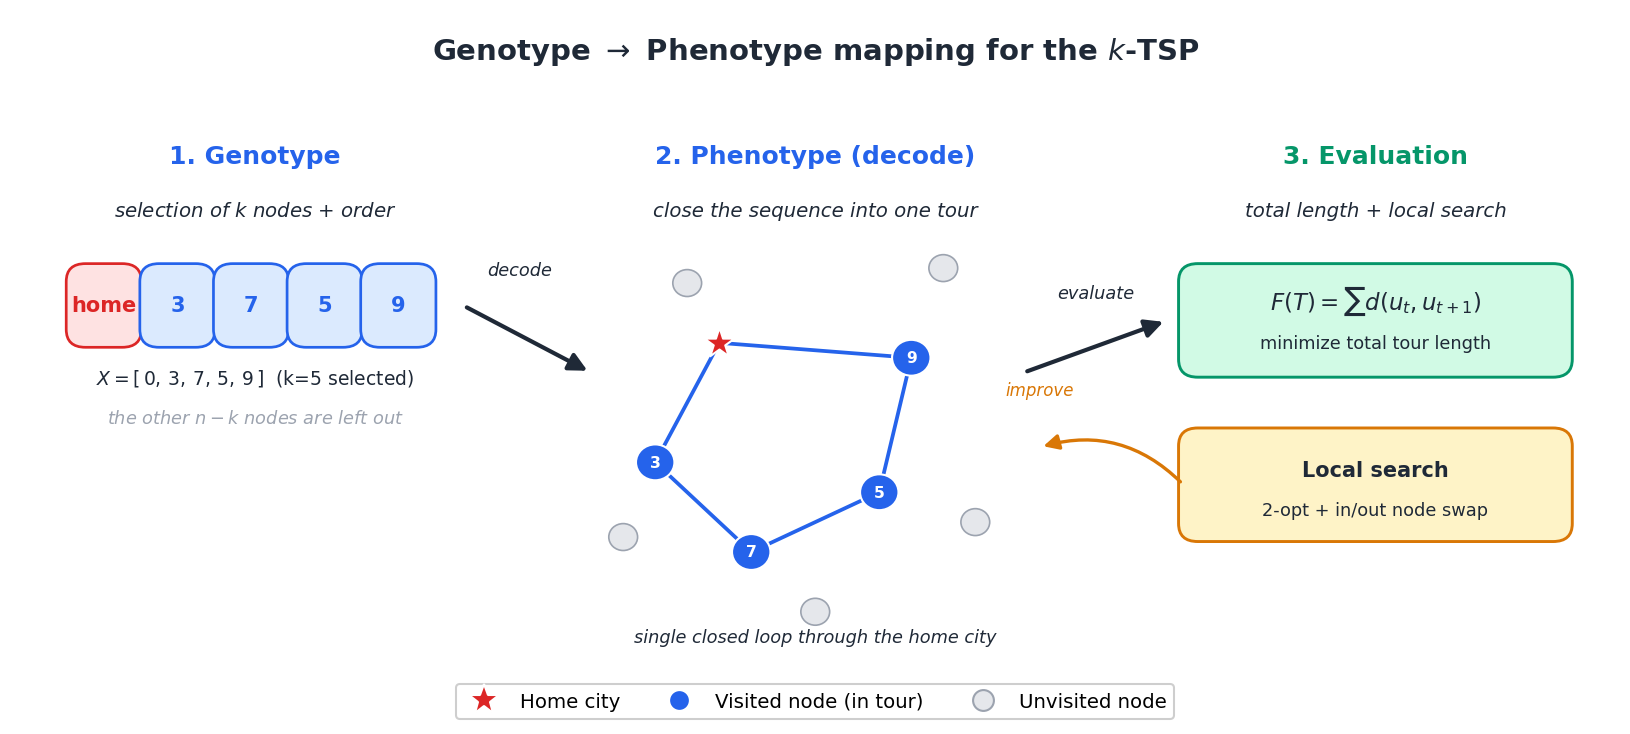
\includegraphics[width=\linewidth]{Genotipo-Fenotipo.png}
    \caption{Genotype$\rightarrow$phenotype flow for the $k$-TSP: the genotype encodes the selected subset of $k$ nodes and their order; decoding closes the sequence into a single tour through the home city, which is then evaluated by its total length $F(T)$ and refined by local search.}
    \label{fig:Genotipo_Fenotipo}
\end{figure}

% ===================== 3. MATHEMATICAL MODEL =====================
\subsection{Mathematical Modeling}

The $k$-TSP must choose \emph{which} $k$ nodes to visit and \emph{in which order}, which makes the search space combinatorial: the number of candidate subsets is $\binom{n-1}{k-1}$ and each admits $(k-1)!/2$ distinct tours. For example, for $n=100$ and $k=50$ the number of subsets alone exceeds $10^{28}$, so exhaustive enumeration is intractable and heuristic/metaheuristic methods are required. Even for the standard TSP, exact resolution of large instances relies on sophisticated branch-and-cut machinery rather than enumeration \cite{applegate2006concorde}.

Let $G=(V,E)$ with $V=\{0,1,\dots,n-1\}$ and node $0$ the home city (depot). We use a single-salesman selective formulation. Two families of binary variables are introduced:
\begin{itemize}
  \item $y_i=1$ if node $i$ is \emph{selected} (visited), $0$ otherwise.
  \item $x_{ij}=1$ if the tour traverses arc $(i,j)$, $0$ otherwise.
\end{itemize}
Ordering variables $u_i$ (Miller--Tucker--Zemlin \cite{miller1960mtz}) eliminate subtours among the selected nodes.

\subsection*{Objective Function}
Minimize the total length of the single tour:
\begin{equation}
\min\ Z = \sum_{i\in V}\sum_{\substack{j\in V\\ j\neq i}} c_{ij}\,x_{ij}.
\end{equation}

\noindent\textbf{Index interpretation:}
\begin{itemize}
    \item $i$: origin node; $j$: destination node; $c_{ij}$: distance from $i$ to $j$.
    \item $x_{ij}=1$ iff the tour goes directly from $i$ to $j$.
\end{itemize}

\subsection*{Constraints}

\noindent\textbf{Number of visited nodes.} Exactly $k$ nodes are selected, including the home city:
\begin{align}
\sum_{i\in V} y_i &= k, & y_0 &= 1.
\end{align}

\noindent\textbf{Degree linked to selection.} Every selected node has exactly one incoming and one outgoing arc; unselected nodes have none:
\begin{align}
\sum_{\substack{j\in V\\ j\neq i}} x_{ij} &= y_i & \forall\, i\in V,\\
\sum_{\substack{j\in V\\ j\neq i}} x_{ji} &= y_i & \forall\, i\in V.
\end{align}
Thus a node is entered and left if and only if it is selected, and the tour visits precisely the $k$ chosen nodes.

\noindent\textbf{Subtour elimination (MTZ over selected nodes).}
\begin{align}
u_0 &= 0,\\
1 \le u_i &\le k-1 & \forall\, i\in V\setminus\{0\},\\
u_i - u_j + (k-1)\,x_{ij} &\le k-2 & \forall\, i,j\in V\setminus\{0\},\ i\neq j.
\end{align}
These constraints (scaled by $k$, the number of visited nodes, rather than $n$) ensure a single closed tour through the home city and forbid disconnected cycles among the selected nodes.

\noindent\textbf{Variable domains.}
\begin{align}
x_{ij} &\in \{0,1\} & \forall\, i\neq j,\\
y_i &\in \{0,1\} & \forall\, i\in V,\\
u_i &\in \mathbb{R}_{\ge 0} & \forall\, i\in V.
\end{align}

This is a \emph{selective} single-tour TSP: it differs from the standard TSP by the selection variables $y_i$ and the cardinality constraint $\sum_i y_i=k$, and from the multiple-TSP by having a single salesman and no route index $k$ on the arc variables. Related selective routing models (orienteering, prize-collecting) share the node-selection mechanism \cite{vansteenwegen2011top,gunawan2016op}; the $k$-TSP fixes the number of visits to exactly $k$ and minimizes length, as defined by Venkatesh et al.\ \cite{venkatesh2018}.

% ===================== 4. SOLUTION (BEFORE TECHNIQUES) =====================
\begin{figure}[H]
    \centering
    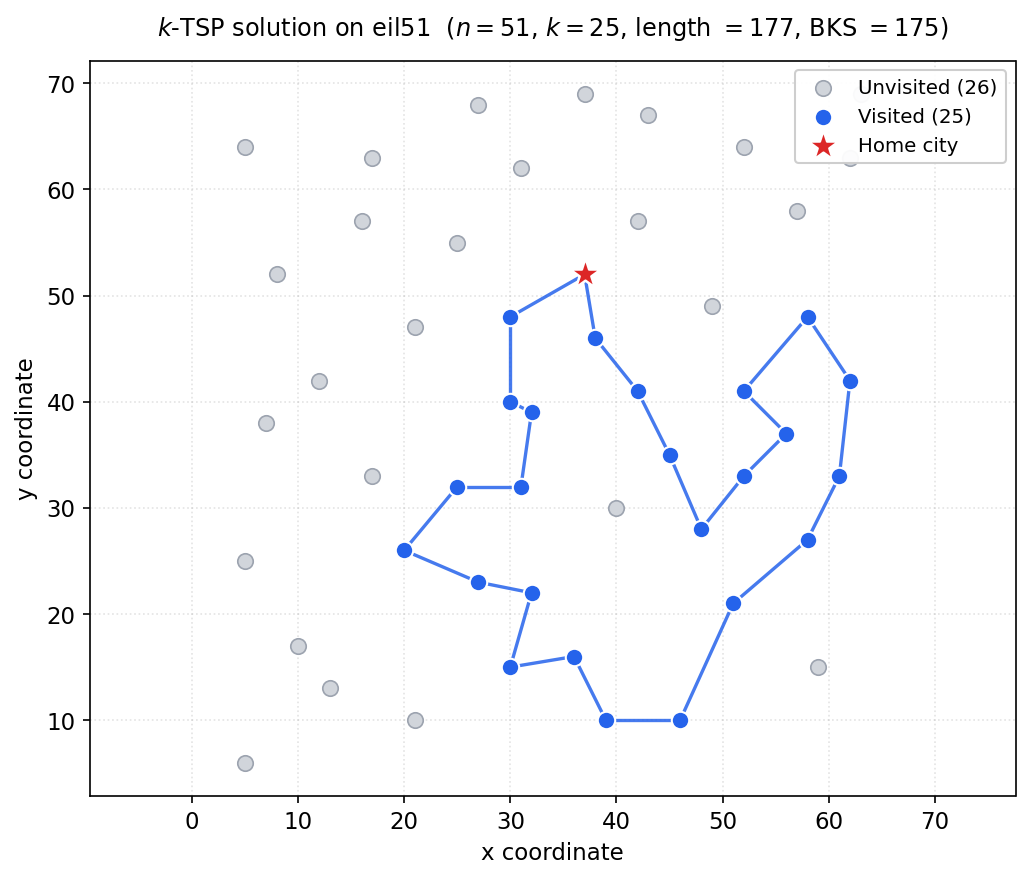
\includegraphics[width=0.65\linewidth]{Graficok-TSP.png}
    \caption{Visualization of a $k$-TSP solution on the \texttt{eil51} instance with $k=25$ ($\lfloor n/2\rfloor$ of the $n=51$ nodes, i.e.\ quartile Q2). A single tour (blue) through the home city (red star) visits the $k$ selected nodes, while the remaining $n-k$ nodes (gray) are left unvisited. The tour shown is the GA solution, of length 177, within $1.1\%$ of the BKS (175); see Table~\ref{tab:resultados_Q2}.}
    \label{fig:eil51_ktsp}
\end{figure}
\noindent\textbf{Interpretation of Fig.~\ref{fig:eil51_ktsp}.}
The tour forms a single closed loop anchored at the home city. Only the selected $k$ nodes belong to the loop; the unvisited nodes lie outside it. After local improvement (2-opt over the cycle and in/out node exchange), the loop becomes shorter and free of crossings, and the selected subset stabilizes around nodes that are cheap to include.

% ===================== 5. SOLUTION TECHNIQUES =====================
\subsection{Solution techniques}\label{sec:soltech}

\paragraph{Greedy (cheapest insertion).}
Starting from the home city, the tour grows by repeatedly inserting the node with the smallest marginal insertion cost,
\[
  \Delta(v,\,u\!\to\!w)=d(u,v)+d(v,w)-d(u,w),
\]
into its best position, until the tour contains $k$ nodes. The result is then refined with 2-opt \cite{croes1958}, whose approximation behaviour and convergence on Euclidean and general instances have been studied in detail \cite{brodowsky2023kopt,heimann2025kopt}. Several deterministic restarts (different second nodes) keep the best tour. Greedy construction is known to be sensitive to the starting choices \cite{gutin2002greedy}, which motivates the restarts. This provides a fast feasible baseline.

\paragraph{GRASP / multi-start.}
Following the Greedy Randomized Adaptive Search Procedure framework \cite{feo1995grasp}, a randomized greedy construction selects, with controlled noise, nodes that are close to the home city, builds a tour, and applies local search (2-opt $+$ in/out exchange). Over many restarts within a time budget, the best tour is retained. Randomization is governed by the fixed seed for reproducibility.

\paragraph{Genetic Algorithm (GA).}
Each individual encodes the selected subset and its order (Section on ADT), in the spirit of the genotype--phenotype evolutionary paradigm \cite{holland1975adaptation}. The population is initialized with random feasible subsets improved by local search. The GA then applies:
\begin{itemize}
  \item \emph{Selection:} binary tournament (favours shorter tours, preserves diversity).
  \item \emph{Crossover:} a subset-aware operator that keeps part of one parent's nodes and completes the child with nodes from the other parent, repairing cardinality.
  \item \emph{Mutation:} swap of two positions and/or exchange of an in-tour node for an out-of-tour node.
  \item \emph{Elitism} and optional 2-opt refinement of offspring.
\end{itemize}
Because crossover and mutation may change \emph{which} nodes are selected, the GA explores the selection space as well as the ordering space, which is essential for the $k$-TSP.

\paragraph{Nearest Neighbor (NN).}
The classic constructive heuristic \cite{rosenkrantz1977}: starting from the home city, the tour is extended by repeatedly moving to the nearest not-yet-visited node until $k$ nodes are selected; the resulting tour is then refined by 2-opt and the in/out exchange. Because the nearest node is chosen deterministically (ties broken by node index), NN is fully reproducible. It is the cheapest method to run in terms of distance evaluations and therefore a natural lower bound on computational effort.

\paragraph{Nearest and Farthest Insertion (NI, FI).}
Two members of the classical insertion family \cite{rosenkrantz1977}. Both start from the edge joining the home city to its nearest node and repeatedly enlarge the tour, always placing the incoming node at the position of minimum insertion cost $\Delta(v,\,u\!\to\!w)$. They differ in \emph{which} node is inserted next: NI selects the outside node \emph{closest} to the current tour, whereas FI selects the outside node \emph{farthest} from it. Farthest Insertion tends to fix the overall shape of the tour early, while Nearest Insertion grows it locally. Both are deterministic and are refined with 2-opt and the in/out exchange.

\paragraph{Random Insertion (RI).}
A stochastic multi-start variant of the insertion family \cite{rosenkrantz1977}: at each step the node to be inserted is chosen \emph{uniformly at random} among the outside nodes and placed at its cheapest position; each construction is improved by local search, and the best tour over many restarts within the budget is retained. Randomization is governed by the fixed seed for reproducibility.

\paragraph{Simulated Annealing (SA).}
A single-solution metaheuristic \cite{kirkpatrick1983}. Starting from a Nearest-Insertion tour, SA explores two neighbourhoods: (i) segment reversal (a 2-opt move that reorders the tour) and (ii) an in/out exchange that swaps a selected node for an unselected one, thereby also searching the selection space. A candidate move with cost change $\Delta$ is always accepted if $\Delta<0$ and otherwise accepted with the Metropolis probability $\exp(-\Delta/T)$; the temperature $T$ is cooled geometrically. SA thus escapes local optima that trap the purely greedy constructions.

\FloatBarrier
\begin{algorithm}[H]
\small
\DontPrintSemicolon
\SetKwInput{KwIn}{Input}
\SetKwInput{KwOut}{Output}
\SetInd{0.5em}{0.8em}
\caption{DCIH (Deterministic Cheapest-Insertion Heuristic) for the $k$-TSP}\label{alg:dci}

\KwIn{nodes $V$, home $0$, count $k$, distances $d$, optional candidate window $w$}
\KwOut{tour $T$ over exactly $k$ nodes minimizing total length}

\tcp{Phase 1 — deterministic cheapest-insertion selection + ordering}
$P \leftarrow V\setminus\{0\}$\;
\If{$w>0$ \textbf{and} $w<|P|$}{$P \leftarrow$ the $w$ nodes nearest to $0$}
$s \leftarrow \arg\min_{v\in P}\,(d(0,v),\,v)$ \tcp*{tie-break by node index}
$T \leftarrow [\,0,\,s\,]$;\quad $P\leftarrow P\setminus\{s\}$\;
\While{$|T| < k$ \textbf{and} $P\neq\varnothing$}{
  \ForEach{$v\in P$ \textnormal{(in increasing index order)}}{
    \ForEach{adjacent pair $(a,b)$ in the cyclic $T$}{
      $\Delta \leftarrow d(a,v)+d(v,b)-d(a,b)$\;
      keep the smallest $(\Delta,\,v,\,\text{position})$
    }
  }
  insert the best $v$ at its best position; remove $v$ from $P$\;
}
\tcp{Phase 2 — deterministic local refinement}
$T \leftarrow \textbf{TwoOptCycle}(T,d)$\;
\Repeat{no improvement}{
  $T,\ \text{changed} \leftarrow \textbf{SwapInOut}(T,d)$ \tcp*{replace an in-tour node by a cheaper out-tour node}
  $T \leftarrow \textbf{TwoOptCycle}(T,d)$\;
}
\Return{$T$}\;
\end{algorithm}
\FloatBarrier

\paragraph{DCIH (Deterministic Cheapest-Insertion Heuristic).}
DCIH is the proposed heuristic of this work. It is intentionally \textbf{simple, explainable, and deterministic}. It attacks the two coupled decisions of the $k$-TSP with a single criterion --- the \emph{marginal insertion cost} --- which selects \emph{which} nodes enter the tour and \emph{where} they are placed (Phase 1), and then refines the tour with 2-opt and an in/out exchange (Phase 2). It differs from the Greedy (cheapest insertion) baseline in two ways: (i) DCIH uses a single deterministic construction with ties broken by node index rather than several deterministic restarts, and (ii) its refinement phase iterates 2-opt together with an in/out node exchange (which can change the selected subset) until no improvement, whereas the Greedy baseline applies only 2-opt over a fixed subset. Because it uses no randomness and breaks ties by node index, DCIH returns exactly the same tour on every run, which makes it fully \emph{reproducible}. The optional candidate window $w$ restricts the candidates to the $w$ nodes nearest the home city to accelerate large instances while remaining deterministic. DCIH prioritizes correctness and reproducibility over winning by chance.

\paragraph{LKH-3 as the reference solver.}
The Lin--Kernighan--Helsgaun solver (LKH, and its extension LKH-3) is among the most effective methods for the TSP and its variants, based on variable-depth local search with sequential gain optimization \cite{Helsgaun,lin1973}. LKH-3~\cite{helsgaun2017lkh3} supports the $k$-TSP natively through the \texttt{SPECIAL} mode and the keyword \texttt{K} (the number of nodes to visit), which makes it the natural choice for a near-optimal reference on the single-tour, node-selection objective. In the present work the reference values (BKS) are exactly those obtained by LKH-3 on the benchmark instances introduced by Pandiri \& Singh~\cite{pandiri2020}, as distributed in Helsgaun's $k$-TSP benchmark package. For several instances these LKH-3 values improve upon the best results originally reported by Pandiri \& Singh, so they constitute the strongest available reference for the comparison.

\begin{table}[H]
\centering
\caption{Solution techniques implemented and compared for the $k$-TSP. LKH-3 (Section~\ref{sec:soltech}) is the source of the reference values (BKS) and is not among the methods run here.}
\label{tab:tecnicas}
\resizebox{\linewidth}{!}{
\begin{tabular}{|p{2.2cm}|p{4.3cm}|p{2.0cm}|}
\hline
\textbf{Method} & \textbf{Main characteristics} & \textbf{Reference} \\ \hline
Greedy (cheapest insertion) &
Builds the tour by minimum marginal insertion until $k$ nodes; 2-opt refinement; fast baseline. &
\cite{croes1958} \\ \hline
GRASP / multi-start &
Randomized greedy construction $+$ local search; best over many restarts; reproducible via fixed seed. &
\cite{feo1995grasp} \\ \hline
Genetic Algorithm (GA) &
Encodes subset $+$ order; tournament, subset-aware crossover, swap/in--out mutation, elitism, 2-opt. &
\cite{holland1975adaptation} \\ \hline
Nearest Neighbor (NN) &
Extends the tour to the nearest unvisited node until $k$; 2-opt $+$ in/out refinement; deterministic. &
\cite{rosenkrantz1977} \\ \hline
Nearest / Farthest Insertion (NI, FI) &
Insertion family; inserts the node closest to (NI) or farthest from (FI) the tour at its cheapest position; deterministic. &
\cite{rosenkrantz1977} \\ \hline
Random Insertion (RI) &
Multi-start insertion with the next node chosen at random; local search; reproducible via fixed seed. &
\cite{rosenkrantz1977} \\ \hline
Simulated Annealing (SA) &
Metropolis acceptance over 2-opt and in/out neighbourhoods with geometric cooling; escapes local optima. &
\cite{kirkpatrick1983} \\ \hline
\textbf{DCIH (proposed)} &
Deterministic cheapest-insertion selection $+$ 2-opt and in/out exchange; fully reproducible. &
--- \\ \hline
\end{tabular}}
\end{table}

% ===================== 6. GENERATION + METRICS =====================
\section{Benchmarks and Evaluation}
\subsection*{Instance generation}
Standard TSPLIB instances~\cite{TSPLIB} provide coordinates and a distance type per instance, enabling evaluation on widely used benchmark cases; all the experiments reported in this work use these TSPLIB instances. The repository additionally supports \textbf{synthetic instances} generated in the plane with nodes drawn from a uniform distribution using a fixed seed (\texttt{seed = 42}); for such instances, coordinates $(x,y)$ are assigned to each node and distances are computed as the Euclidean norm:
\[
  d_{ij}=\sqrt{(x_i-x_j)^2+(y_i-y_j)^2}.
\]
For each instance, three values of the number of nodes to visit $k$ are evaluated, following the $k$-TSP benchmark of Pandiri \& Singh~\cite{pandiri2020}: $k=\lfloor n/4\rfloor$ (Q1), $k=\lfloor n/2\rfloor$ (Q2), and $k=\lfloor 3n/4\rfloor$ (Q3). This setup allows analysing performance across sizes and geometric configurations.

\subsection*{Metrics}
The analysed metrics are:
\begin{itemize}
    \item \textbf{Total tour length}: the length of the single closed tour over the $k$ selected nodes (the objective to minimize).
    \item \textbf{Relative GAP}: $100\cdot(\text{length}-\text{BKS})/\text{BKS}$, where BKS is the best-known value obtained by LKH-3~\cite{Helsgaun} on the benchmark instances of Pandiri \& Singh~\cite{pandiri2020} for the instance and value of $k$.
\end{itemize}
Selective routing problems such as the Orienteering Problem and the Prize-Collecting TSP share the node-selection mechanism and are natural points of comparison for the $k$-TSP objective \cite{vansteenwegen2011top}.

% ===================== 8. EXPERIMENTAL ENVIRONMENT =====================
\section{Experimental Environment}
All experiments were executed on \textbf{Google Colab}, a cloud notebook environment with reproducible resources:
\begin{itemize}
    \item \textbf{Environment:} Google Colab cloud notebook.
    \item \textbf{CPU:} Intel Xeon (virtualized, 2--4 cores).
    \item \textbf{RAM:} 12--16 GB depending on the session.
    \item \textbf{OS:} Linux (Ubuntu, virtualized in Colab).
    \item \textbf{Languages and libraries:} Python 3.10 with \texttt{numpy}, \texttt{pandas}, \texttt{matplotlib}, \texttt{requests}.
\end{itemize}
This environment allows consistent measurement of total tour length, and its public availability supports replication.

% ===================== 9. ROUTE ANALYSIS =====================
\section{Analysis of Generated Tours}
\subsection*{Solution patterns (Greedy vs.\ GRASP vs.\ GA vs.\ DCIH)}

The tours produced for the $k$-TSP are single closed loops through the home city over a selected subset of $k$ nodes. The constructive methods (Greedy, DCIH) tend to select nodes that are cheap to insert, yielding compact loops, while GRASP and the GA explore alternative subsets that can shorten the tour further. After 2-opt and the in/out exchange, crossings are removed and the selected subset stabilizes. The LKH-3 tours, which define the BKS reference here, attain the shortest known lengths and serve as the near-optimal baseline against which all methods are measured.

\section{Comparison of Results}
This section reports the experimental results of the implemented methods on the $k$-TSP objective (\emph{total tour length}, lower is better): the greedy cheapest-insertion baseline, GRASP/multi-start, the genetic algorithm (GA), and the proposed deterministic heuristic \textbf{DCIH} (Deterministic Cheapest-Insertion Heuristic). The experiments use 38 standard TSPLIB instances and follow the $k$-TSP benchmark of Pandiri \& Singh~\cite{pandiri2020}, which defines three values of $k$ per instance: \textbf{Q1} ($k=\lfloor n/4\rfloor$), \textbf{Q2} ($k=\lfloor n/2\rfloor$), and \textbf{Q3} ($k=\lfloor 3n/4\rfloor$). Each result is compared against the best-known value (BKS) obtained by LKH-3~\cite{Helsgaun} on the benchmark instances of Pandiri \& Singh~\cite{pandiri2020} for the corresponding quartile, and the relative GAP is computed as $\mathrm{GAP}\%=100\,(\text{length}-\text{BKS})/\text{BKS}$.

Table~\ref{tab:resumen_gap} summarizes the average GAP per method and quartile. Tables~\ref{tab:resultados_Q1}, \ref{tab:resultados_Q2}, and \ref{tab:resultados_Q3} give the per-instance lengths for Q1, Q2, and Q3 respectively; values in bold coincide with the LKH-3 BKS.

\begin{table}[htbp]
\centering
\caption{Average relative GAP (\%) vs the LKH-3 BKS, per method and quartile. Lower is better. Q1: $k=\lfloor n/4\rfloor$, Q2: $k=\lfloor n/2\rfloor$, Q3: $k=\lfloor 3n/4\rfloor$. Computed over 38 TSPLIB instances.}
\label{tab:resumen_gap}
\begin{tabular}{|l|c|c|c|}
\hline
\textbf{Method} & \textbf{Q1 GAP\%} & \textbf{Q2 GAP\%} & \textbf{Q3 GAP\%} \\
\hline
Greedy & 14.92 & 15.46 & 14.36 \\
GRASP & 21.63 & 22.79 & 20.23 \\
GA & 30.94 & 23.17 & 15.02 \\
\textbf{DCIH} & 19.94 & 23.62 & 20.59 \\
\hline
\end{tabular}
\end{table}

\begin{table*}[htbp]
\centering
\caption{Results for the $k$-TSP, quartile Q1 ($k\approx n/4$). Total tour length per method; BKS = best-known value obtained by LKH-3 on the benchmark instances of Pandiri \& Singh. Values in \textbf{bold} match the BKS.}
\label{tab:resultados_Q1}
{\footnotesize\setlength{\tabcolsep}{4.5pt}\renewcommand{\arraystretch}{0.95}%
\begin{tabular}{|l|c|c|c|c|c|c|c|}
\hline
\textbf{Instance} & \textbf{$n$} & \textbf{$k$} & \textbf{Greedy} & \textbf{GRASP} & \textbf{GA} & \textbf{DCIH} & \textbf{BKS} \\
\hline
att48 & 48 & 12 & 2363 & 2315 & \textbf{1925} & 2363 & 1925 \\
eil51 & 51 & 12 & 88 & 90 & \textbf{82} & 83 & 82 \\
berlin52 & 52 & 13 & \textbf{679} & 709 & \textbf{679} & 735 & 679 \\
st70 & 70 & 17 & 140 & \textbf{120} & 125 & \textbf{120} & 120 \\
eil76 & 76 & 19 & 107 & 122 & \textbf{102} & 129 & 102 \\
pr76 & 76 & 19 & 23929 & 25966 & 24510 & 28089 & 23450 \\
kroA100 & 100 & 25 & 5285 & 5778 & 5102 & 5885 & 4931 \\
kroB100 & 100 & 25 & 5232 & 4549 & 4906 & 4676 & 4305 \\
kroC100 & 100 & 25 & 5834 & 5835 & 5684 & 6577 & 4964 \\
kroD100 & 100 & 25 & 4787 & 5125 & 5411 & 5449 & 4762 \\
kroE100 & 100 & 25 & 4660 & 4899 & 5336 & 4587 & 3905 \\
eil101 & 101 & 25 & 124 & 144 & 108 & 154 & 107 \\
lin105 & 105 & 26 & 3534 & \textbf{2606} & \textbf{2606} & 2881 & 2606 \\
pr107 & 107 & 26 & 10937 & 8615 & \textbf{8443} & 9032 & 8443 \\
pr124 & 124 & 31 & 15508 & 15173 & 17833 & 16282 & 14325 \\
bier127 & 127 & 31 & 11664 & 11628 & 11234 & 11994 & 10619 \\
ch130 & 130 & 32 & 1296 & 1408 & 1346 & 1373 & 1130 \\
pr136 & 136 & 34 & 24136 & 23620 & 26164 & 24235 & 21116 \\
gr137 & 137 & 34 & 18514 & 18943 & 18101 & 18496 & 17399 \\
ch150 & 150 & 37 & 1525 & 1541 & 1652 & 1369 & 1276 \\
kroA150 & 150 & 37 & 6362 & 7483 & 6593 & 7286 & 5690 \\
kroB150 & 150 & 37 & 6486 & 7446 & 7306 & 7802 & 5812 \\
rat195 & 195 & 48 & 627 & 607 & 659 & 604 & 554 \\
kroA200 & 200 & 50 & 7369 & 7327 & 8704 & 7998 & 6154 \\
kroB200 & 200 & 50 & 7145 & 7559 & 8901 & 7979 & 6016 \\
ts225 & 225 & 56 & 30478 & 32441 & 40656 & 35943 & 28828 \\
tsp225 & 225 & 56 & 974 & 1175 & 1215 & 1080 & 913 \\
pr226 & 226 & 56 & 25609 & 26550 & 32748 & 25781 & 20033 \\
gr229 & 229 & 57 & 20110 & 26053 & 27002 & 20650 & 18555 \\
gil262 & 262 & 65 & 661 & 680 & 755 & 792 & 541 \\
pr264 & 264 & 66 & 9729 & 12551 & 22834 & 9581 & 9232 \\
a280 & 280 & 70 & 763 & 775 & 888 & 702 & 649 \\
pr299 & 299 & 74 & 13585 & 14680 & 14785 & 14440 & 11077 \\
lin318 & 318 & 79 & 10089 & 9937 & 11974 & 10753 & 8544 \\
rd400 & 400 & 100 & 3830 & 4264 & 4675 & 3897 & 3091 \\
fl417 & 417 & 104 & 2187 & 2896 & 6125 & 2129 & 1831 \\
pr439 & 439 & 109 & 22976 & 34718 & 24900 & 29358 & 19751 \\
pcb442 & 442 & 110 & 13533 & 14836 & 14745 & 13818 & 10932 \\
\hline
\end{tabular}}
\end{table*}

\begin{table*}[htbp]
\centering
\caption{Results for the $k$-TSP, quartile Q2 ($k\approx n/2$). Total tour length per method; BKS = best-known value obtained by LKH-3 on the benchmark instances of Pandiri \& Singh. Values in \textbf{bold} match the BKS.}
\label{tab:resultados_Q2}
{\footnotesize\setlength{\tabcolsep}{4.5pt}\renewcommand{\arraystretch}{0.95}%
\begin{tabular}{|l|c|c|c|c|c|c|c|}
\hline
\textbf{Instance} & \textbf{$n$} & \textbf{$k$} & \textbf{Greedy} & \textbf{GRASP} & \textbf{GA} & \textbf{DCIH} & \textbf{BKS} \\
\hline
att48 & 48 & 24 & 4740 & 4280 & \textbf{3603} & 4896 & 3603 \\
eil51 & 51 & 25 & 193 & 191 & 177 & 198 & 175 \\
berlin52 & 52 & 26 & 2016 & 2031 & \textbf{1874} & 2269 & 1874 \\
st70 & 70 & 35 & 297 & 294 & 280 & 302 & 260 \\
eil76 & 76 & 38 & 247 & 261 & 229 & 249 & 213 \\
pr76 & 76 & 38 & 42968 & 51311 & 42749 & 51378 & 41248 \\
kroA100 & 100 & 50 & 10198 & 10818 & 10913 & 12532 & 9184 \\
kroB100 & 100 & 50 & 10170 & 9380 & 10923 & 11557 & 9096 \\
kroC100 & 100 & 50 & 11206 & 10657 & 10483 & 12916 & 9457 \\
kroD100 & 100 & 50 & 9990 & 10864 & 9956 & 11438 & 8719 \\
kroE100 & 100 & 50 & 10680 & 10021 & 11057 & 11061 & 9097 \\
eil101 & 101 & 50 & 255 & 310 & 263 & 276 & 227 \\
lin105 & 105 & 52 & 6131 & 6677 & 6193 & 6066 & 5848 \\
pr107 & 107 & 53 & 18211 & 18576 & 30547 & 18564 & 18028 \\
pr124 & 124 & 62 & 26299 & 32871 & 35569 & 28151 & 22998 \\
bier127 & 127 & 63 & 33091 & 28446 & 30447 & 28900 & 25761 \\
ch130 & 130 & 65 & 2802 & 2878 & 2853 & 3145 & 2408 \\
pr136 & 136 & 68 & 48664 & 54666 & 50574 & 50223 & 46414 \\
gr137 & 137 & 68 & 33447 & 33451 & 35752 & 32687 & 29231 \\
ch150 & 150 & 75 & 3245 & 3478 & 3368 & 3511 & 2760 \\
kroA150 & 150 & 75 & 14172 & 14956 & 14481 & 15061 & 11496 \\
kroB150 & 150 & 75 & 13616 & 14350 & 13147 & 15202 & 11357 \\
rat195 & 195 & 97 & 1234 & 1222 & 1298 & 1231 & 1100 \\
kroA200 & 200 & 100 & 14820 & 14628 & 15620 & 16045 & 12372 \\
kroB200 & 200 & 100 & 14781 & 15145 & 15478 & 16395 & 12338 \\
ts225 & 225 & 112 & 69383 & 70307 & 71421 & 74223 & 56828 \\
tsp225 & 225 & 112 & 1967 & 2169 & 2130 & 2105 & 1708 \\
pr226 & 226 & 113 & 42073 & 50460 & 47965 & 49551 & 36720 \\
gr229 & 229 & 114 & 47860 & 53016 & 51139 & 49566 & 39618 \\
gil262 & 262 & 131 & 1221 & 1341 & 1288 & 1382 & 993 \\
pr264 & 264 & 132 & 24137 & 24045 & 32922 & 23423 & 22644 \\
a280 & 280 & 140 & 1355 & 1511 & 1530 & 1362 & 1231 \\
pr299 & 299 & 149 & 25833 & 26669 & 27046 & 26930 & 22390 \\
lin318 & 318 & 159 & 20419 & 22531 & 22441 & 20949 & 15916 \\
rd400 & 400 & 200 & 7941 & 8419 & 8082 & 7922 & 6350 \\
fl417 & 417 & 208 & 5786 & 6976 & 8070 & 6162 & 5436 \\
pr439 & 439 & 219 & 42307 & 57751 & 53256 & 55146 & 35404 \\
pcb442 & 442 & 221 & 25747 & 30954 & 29366 & 27938 & 22537 \\
\hline
\end{tabular}}
\end{table*}

\begin{table*}[htbp]
\centering
\caption{Results for the $k$-TSP, quartile Q3 ($k\approx 3n/4$). Total tour length per method; BKS = best-known value obtained by LKH-3 on the benchmark instances of Pandiri \& Singh. Values in \textbf{bold} match the BKS.}
\label{tab:resultados_Q3}
{\footnotesize\setlength{\tabcolsep}{4.5pt}\renewcommand{\arraystretch}{0.95}%
\begin{tabular}{|l|c|c|c|c|c|c|c|}
\hline
\textbf{Instance} & \textbf{$n$} & \textbf{$k$} & \textbf{Greedy} & \textbf{GRASP} & \textbf{GA} & \textbf{DCIH} & \textbf{BKS} \\
\hline
att48 & 48 & 36 & 6877 & 6727 & 7215 & 6816 & 6563 \\
eil51 & 51 & 38 & 303 & 304 & 298 & 316 & 287 \\
berlin52 & 52 & 39 & 4549 & 4220 & 4442 & 4627 & 4174 \\
st70 & 70 & 52 & 463 & 459 & 460 & 495 & 428 \\
eil76 & 76 & 57 & 373 & 396 & 359 & 366 & 335 \\
pr76 & 76 & 57 & 66580 & 72594 & 66337 & 70861 & 64142 \\
kroA100 & 100 & 75 & 16744 & 15900 & 15408 & 18142 & 14379 \\
kroB100 & 100 & 75 & 16204 & 16531 & 15937 & 18413 & 14680 \\
kroC100 & 100 & 75 & 17252 & 16900 & 15228 & 18390 & 13892 \\
kroD100 & 100 & 75 & 16478 & 15947 & 16038 & 17539 & 14058 \\
kroE100 & 100 & 75 & 16965 & 17114 & 16067 & 17418 & 14622 \\
eil101 & 101 & 75 & 445 & 440 & 423 & 458 & 386 \\
lin105 & 105 & 78 & 9503 & 10157 & 10363 & 9388 & 8983 \\
pr107 & 107 & 80 & 37637 & 38231 & 37683 & 38745 & 36292 \\
pr124 & 124 & 93 & 40183 & 49268 & 45357 & 41170 & 39008 \\
bier127 & 127 & 95 & 51088 & 56391 & 58880 & 53130 & 49680 \\
ch130 & 130 & 97 & 4439 & 4515 & 4347 & 4712 & 3876 \\
pr136 & 136 & 102 & 74436 & 78605 & 71585 & 78397 & 67910 \\
gr137 & 137 & 102 & 51562 & 52044 & 47647 & 51456 & 43670 \\
ch150 & 150 & 112 & 5005 & 5105 & 4878 & 5199 & 4366 \\
kroA150 & 150 & 112 & 20542 & 21174 & 20284 & 21792 & 17395 \\
kroB150 & 150 & 112 & 19655 & 21015 & 18925 & 21390 & 16879 \\
rat195 & 195 & 146 & 1846 & 1913 & 1910 & 1850 & 1667 \\
kroA200 & 200 & 150 & 22680 & 24633 & 22530 & 24181 & 19211 \\
kroB200 & 200 & 150 & 23400 & 23138 & 22249 & 24860 & 18898 \\
ts225 & 225 & 168 & 102616 & 102059 & 100789 & 104534 & 85656 \\
tsp225 & 225 & 168 & 2983 & 3248 & 3132 & 3188 & 2624 \\
pr226 & 226 & 169 & 60502 & 68527 & 56507 & 78670 & 47142 \\
gr229 & 229 & 171 & 73199 & 78235 & 89517 & 74146 & 64457 \\
gil262 & 262 & 196 & 1875 & 1956 & 1856 & 1940 & 1551 \\
pr264 & 264 & 198 & 38240 & 43109 & 41956 & 42020 & 34346 \\
a280 & 280 & 210 & 2050 & 2184 & 2161 & 2188 & 1845 \\
pr299 & 299 & 224 & 39460 & 42648 & 38408 & 39938 & 32738 \\
lin318 & 318 & 238 & 32561 & 34576 & 32307 & 32867 & 25303 \\
rd400 & 400 & 300 & 11981 & 12791 & 11803 & 11937 & 9972 \\
fl417 & 417 & 312 & 9853 & 12030 & 9571 & 11377 & 7930 \\
pr439 & 439 & 329 & 66325 & 82830 & 83969 & 76532 & 58006 \\
pcb442 & 442 & 331 & 40390 & 42461 & 41026 & 40952 & 34358 \\
\hline
\end{tabular}}
\end{table*}

\subsection*{Analysis}
The results are consistent across the whole benchmark: no method ever beats the LKH-3 BKS (no negative GAP appears), which confirms that all techniques are solving the same problem (the $k$-TSP) and that the reference is consistent. Some method matches the LKH-3 BKS on a handful of small instances (7 instances in Q1, 2 in Q2, and none in Q3); these matches are almost always attained by the GA (6 of the 7 in Q1, both in Q2).

A clear pattern emerges with the number of visited nodes $k$. The greedy cheapest-insertion baseline is the most robust method across the whole range of $k$, attaining the lowest average GAP in every quartile: $14.9\%$ in Q1, $15.5\%$ in Q2, and $14.4\%$ in Q3. For small $k$ (\textbf{Q1}, $k\approx n/4$) Greedy leads clearly, ahead of DCIH ($19.9\%$), GRASP ($21.6\%$), and GA ($30.9\%$); the GA is penalized here by a few large outliers (e.g.\ \texttt{fl417} and \texttt{pr264}), where its exploration of subsets occasionally selects expensive nodes when only a quarter of them are visited.

As $k$ grows, the \emph{genetic algorithm} closes the gap with the constructive methods. In \textbf{Q3} ($k\approx 3n/4$) the GA reaches an average GAP of $15.0\%$, essentially tied with Greedy ($14.4\%$) and well below GRASP ($20.2\%$) and DCIH ($20.6\%$); moreover the GA becomes the most frequent per-instance winner in this regime (best or tied in $23/38$ instances, against $10/38$ for Greedy). With larger tours the ordering decision dominates and the GA's crossover and 2-opt refinement pay off, even though its average is not lower than Greedy's. \textbf{Q2} ($k\approx n/2$) is a transition regime: Greedy remains best on average ($15.5\%$), while GRASP, GA, and DCIH are clustered around $22$--$24\%$ ($22.8\%$, $23.2\%$, and $23.6\%$ respectively).

\paragraph{On DCIH (the proposed heuristic).}
DCIH is competitive and stable, with average GAPs of $19.9\%$, $23.6\%$, and $20.6\%$ across the three quartiles. For small $k$ (Q1) it is clearly the second-best method, behind Greedy and ahead of both GRASP and GA; for Q2 and Q3 it sits in the same band as the other non-greedy constructive heuristics. It does not lead the ranking, which is the expected trade-off for its design goal: DCIH is fully \emph{deterministic} and therefore exactly reproducible (re-running it yields identical tours), whereas GRASP and GA rely on randomization and a time budget. In other words, DCIH trades a few points of average quality for guaranteed reproducibility and a single, fast, parameter-free run. This makes it a reliable baseline whose results can be verified exactly, which is valuable for reproducible experimentation.

\paragraph{Summary.}
Across the full range of $k$, the greedy cheapest-insertion baseline is the strongest method on average, while the genetic algorithm catches up and becomes the most frequent per-instance winner only for large $k$ (Q3). DCIH provides a deterministic, reproducible alternative of comparable quality throughout: it is the clear second-best method for small $k$ (Q1) and stays within the same band as the other non-greedy constructive heuristics for larger $k$. All methods stay within a moderate GAP of the LKH-3 BKS, confirming that the implementation solves the $k$-TSP correctly across the full range of $k$.

% ===================== 11. CONCLUSIONS =====================
% ===================== ANYTIME BENCHMARKING (Weise 2014) =====================
% Resultados sobre las 38 instancias TSPLIB reales (paquete oficial k-TSP,
% referencia LKH-3). Figuras requeridas junto al .tex:
%   01_progreso_agregado.png, 02_ecdf_agregado.png, 03_ert_vs_meta.png
% Regenerable con benchmark_weise/run_real.py (--aggregate).
\section{Anytime Evaluation of the Heuristics}\label{sec:anytime}

The end-of-run comparison (Tables~\ref{tab:resumen_gap}--\ref{tab:resultados_Q3})
reports a single value per method. However, the greedy cheapest-insertion
baseline, GRASP and the genetic algorithm are \emph{anytime} algorithms: they
keep a feasible incumbent that improves with more computation, so the stopping
point is an arbitrary choice of the experimenter and a single snapshot can hide
which method is preferable under a given budget~\cite{weise2014benchmarking}. To
make the comparison budget-aware and reproducible, we complement the end-of-run
tables with the anytime benchmarking procedure of
Weise~\textit{et~al.}~\cite{weise2014benchmarking}, run on the \emph{same} 38
TSPLIB instances and the same three quartiles of $k$, using the LKH-3 value as the
reference.

\subsection{Machine-independent time and normalized error}
Following~\cite{weise2014benchmarking}, we replace wall-clock time (which depends
on machine, language and load) by a \emph{machine-independent} measure: the number
of \emph{distance evaluations} (DE), i.e.\ accesses to the distance matrix. Every
run emits \emph{log points} $(\mathrm{DE},\,\text{length})$ each time it produces
or updates a solution, recording the full optimization \emph{trajectory} instead
of only its endpoint. Quality is the normalized error
\begin{equation}
F \;=\; \frac{\text{length}}{\text{BKS}} \;-\; 1 ,
\end{equation}
so $F=0$ is the LKH-3 best-known value and, e.g., $F=0.20$ a tour $20\%$ longer.
To aggregate across instances of different size $n$, the DE axis is scaled by
$n^2$, as suggested in~\cite{weise2014benchmarking}. Each stochastic method is run
$10$ times per instance and quartile; DCIH is deterministic (a single run). All
methods share the same budget of $15\,n^2$ distance evaluations.

\subsection{Progress curves, ERT and ECDF}
From the logged trajectories we build three standard views:
\emph{(i)}~\textbf{progress curves}, the median (over runs) best-so-far error $F$
versus the scaled DE (Fig.~\ref{fig:anytime_progress});
\emph{(ii)}~the \textbf{Estimated Running Time} $\mathrm{ERT}(F_t)$, the expected
DE to reach a target error $F_t$, with the restart estimator
$\mathrm{ERT}=(\sum_i \mathrm{DE}_i)/\#\text{successes}$ where failed runs
contribute the full budget (Fig.~\ref{fig:anytime_ert}); and
\emph{(iii)}~the \textbf{Empirical Cumulative Distribution Function}
$\mathrm{ECDF}(F_t)$, the fraction of runs that reached $F_t$ by a given DE
(Fig.~\ref{fig:anytime_ecdf}). As a scalar summary of each curve we use the area
under it (AUC) on the logarithmic DE axis.

\begin{figure}[t]
    \centering
    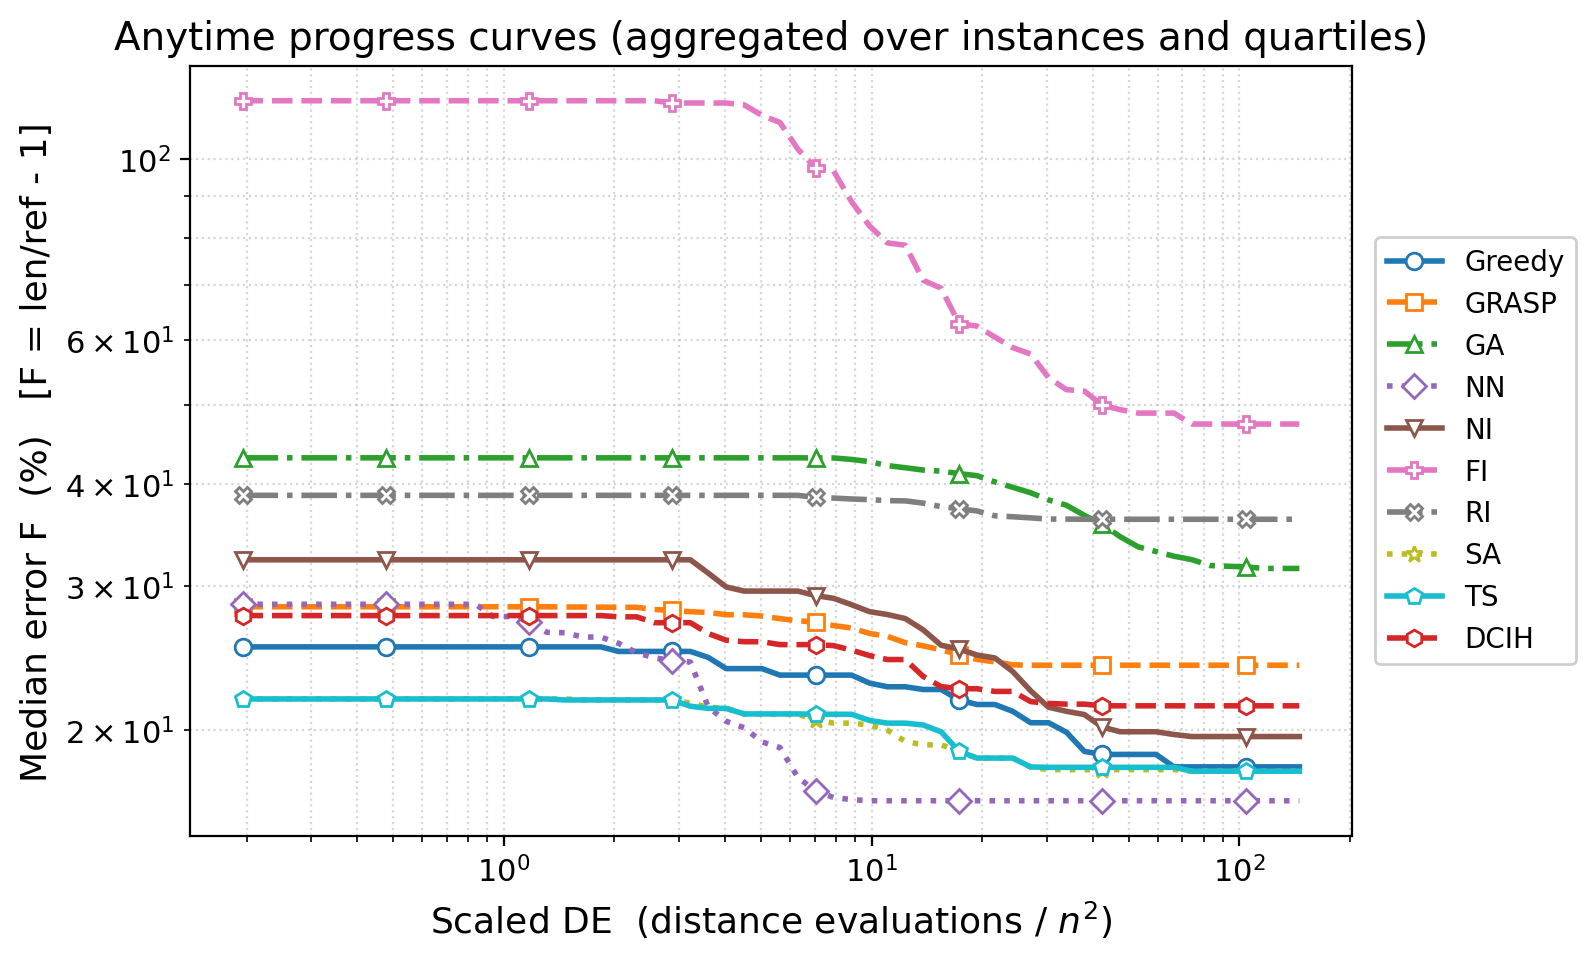
\includegraphics[width=\linewidth]{01_progreso_agregado.png}
    \caption{Anytime \textbf{progress curves} aggregated over the 38 TSPLIB
    instances and the three quartiles of $k$: median best-so-far error $F$ (\%)
    versus the machine-independent time (distance evaluations scaled by $n^2$).
    Lower and earlier is better. The greedy cheapest-insertion baseline dominates
    at every budget, DCIH follows closely and deterministically, and the genetic
    algorithm starts far worse and is still descending at the end of the budget,
    indicating it has not yet converged.}
    \label{fig:anytime_progress}
\end{figure}

\begin{figure}[t]
    \centering
    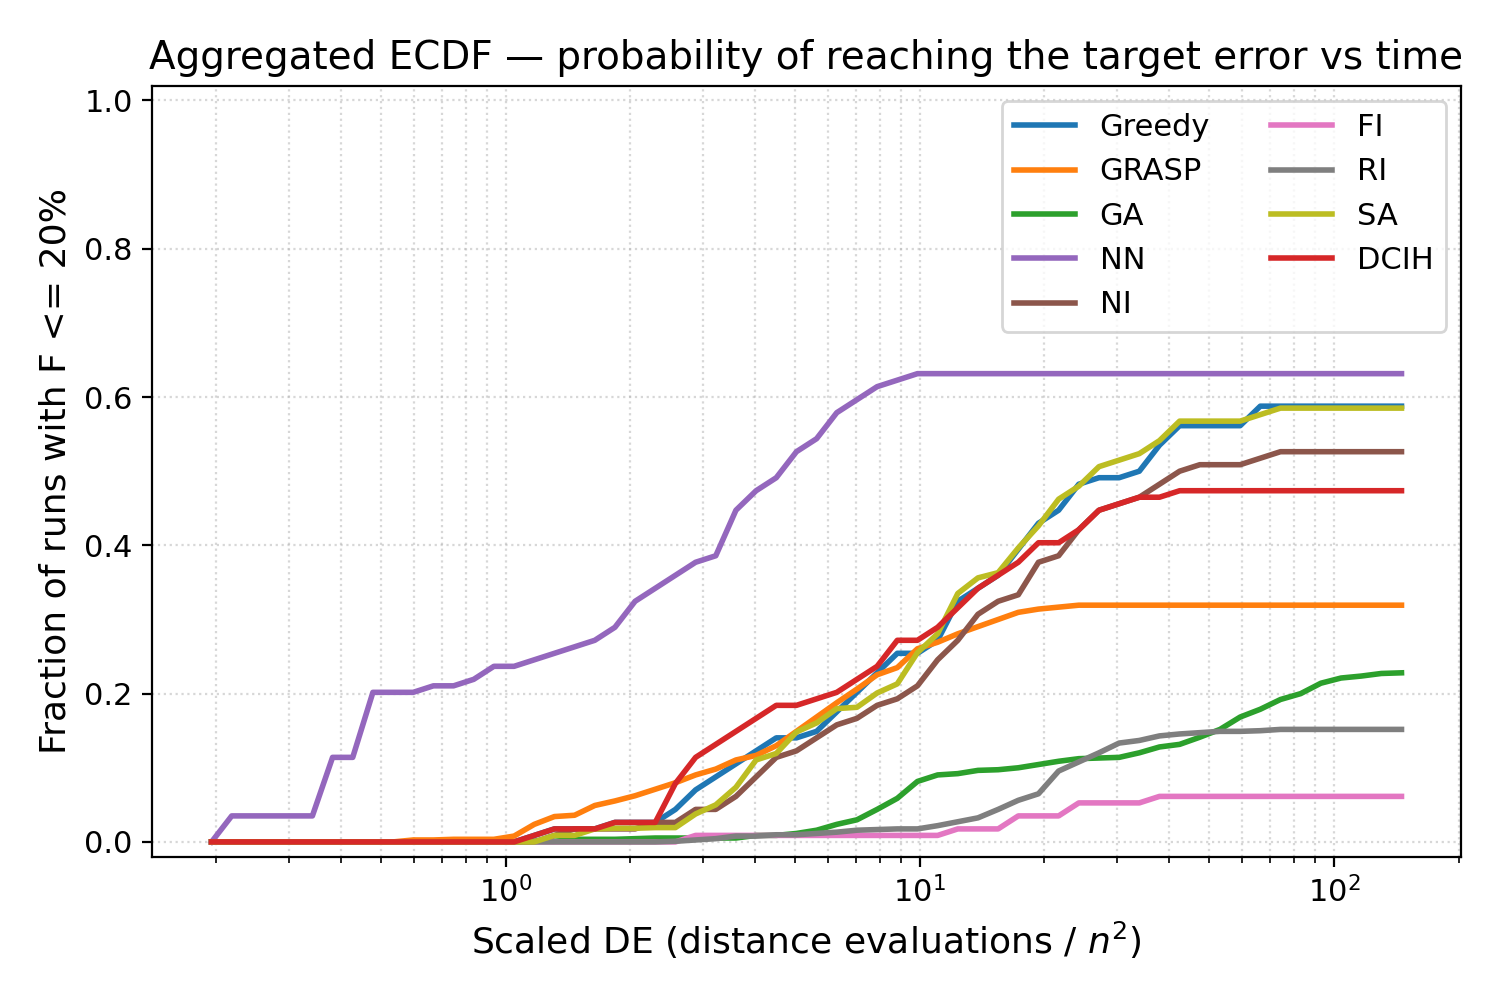
\includegraphics[width=\linewidth]{02_ecdf_agregado.png}
    \caption{Aggregated \textbf{ECDF} for the target error $F_t=20\%$: fraction of
    runs (over instances, quartiles and repetitions) that reach a tour within
    $20\%$ of the LKH-3 reference as a function of the scaled distance evaluations.
    Greedy attains the target in the largest fraction of runs ($\approx59\%$),
    followed by DCIH ($\approx48\%$), GRASP ($\approx32\%$) and GA ($\approx23\%$).}
    \label{fig:anytime_ecdf}
\end{figure}

\begin{figure}[t]
    \centering
    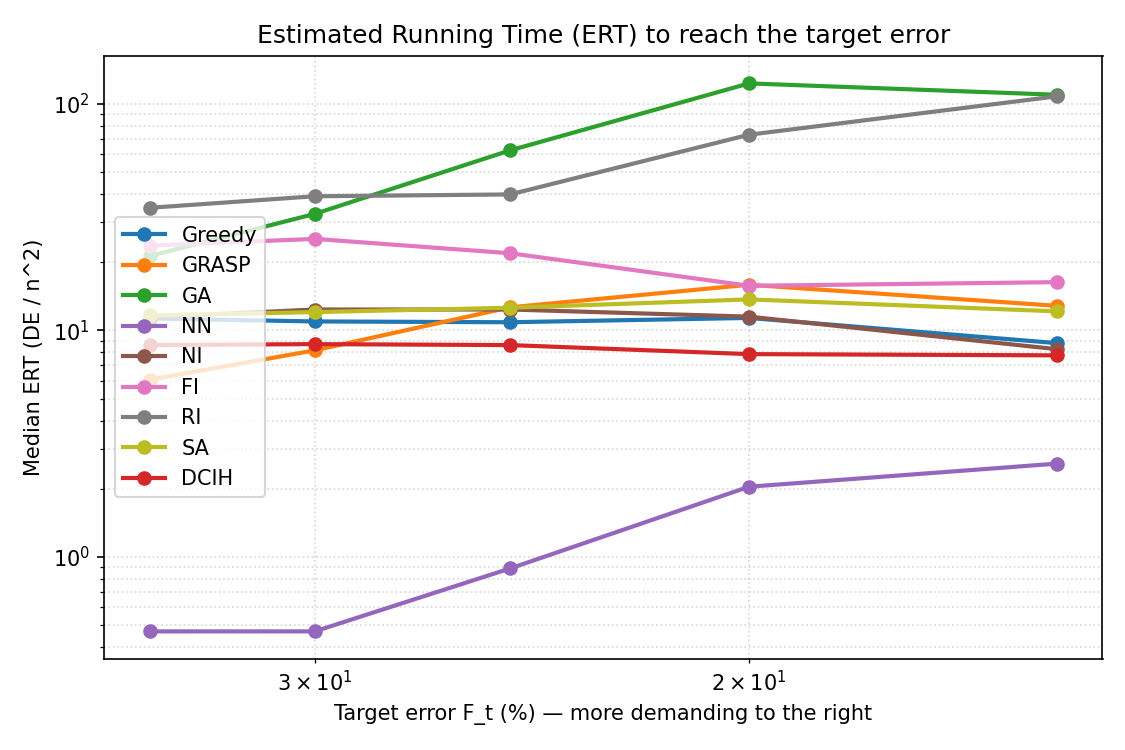
\includegraphics[width=\linewidth]{03_ert_vs_meta.png}
    \caption{Median \textbf{ERT} (scaled distance evaluations, $\mathrm{DE}/n^2$)
    to reach each target error $F_t$ (from $35\%$ down to $15\%$; more demanding to
    the right). Greedy and DCIH reach a given quality with the least computation,
    while the genetic algorithm needs about an order of magnitude more.}
    \label{fig:anytime_ert}
\end{figure}

\subsection{Aggregated ranking}
To condense the views into a single conclusion, on every instance/quartile we rank
the methods by four criteria --- final error, AUC of the progress curve, AUC of the
ECDF, and $\mathrm{ERT}$ at $F_t=20\%$ --- and aggregate by the median rank,
obtaining the global ranking of Table~\ref{tab:anytime_ranking}~\cite{weise2014benchmarking}.
The anytime view is consistent with the end-of-run results
(Tables~\ref{tab:resumen_gap}--\ref{tab:resultados_Q3}): under a fixed
machine-independent budget the greedy cheapest-insertion heuristic is the most
robust method, DCIH provides a competitive \emph{deterministic} trajectory (no
variance across runs), GRASP follows, and the population-based genetic algorithm
converges most slowly and ranks last within this budget. This does not contradict
the advantage of the GA for large $k$: its median error decreases fastest late in
the run (Fig.~\ref{fig:anytime_progress}) and, at the largest quartile Q3, it
approaches the greedy baseline, in agreement with the end-of-run comparison.

\begin{table}[htbp]
\centering
\caption{Anytime \textbf{global ranking} (median rank, lower is better) aggregating
four criteria over the 38 TSPLIB instances and the three quartiles of $k$, with the
LKH-3 value as reference.}
\label{tab:anytime_ranking}
\begin{tabular}{|l|c|c|c|c|c|}
\hline
\textbf{Method} & \textbf{Final} & \textbf{AUC} & \textbf{AUC} & \textbf{ERT} & \textbf{Global} \\
                & \textbf{$F$}   & \textbf{prog.}& \textbf{ECDF}& \textbf{@20\%}& \textbf{rank} \\
\hline
\textbf{Greedy} & 1.5 & 1.0 & 2.5 & 2.50 & \textbf{2.00} \\
DCIH            & 2.0 & 2.0 & 2.5 & 2.50 & 2.25 \\
GRASP           & 3.0 & 3.0 & 2.5 & 2.75 & 2.88 \\
GA              & 4.0 & 4.0 & 3.0 & 3.00 & 3.50 \\
\hline
\end{tabular}
\end{table}

\subsection{Reproducibility}
The procedure is automated in the companion module \texttt{benchmark\_weise}
(Python): it instruments the four methods with the DE counter and log points, reads
the standard TSPLIB instances and the LKH-3 references from the official k-TSP
package, and regenerates every figure and table with a single command. Because the
time axis is machine-independent and the random seeds are fixed, the anytime
results are reproducible across machines.

\section{Conclusions and Future Work}
The $k$-TSP is a selective routing problem: choosing exactly $k$ nodes (including the home city) and ordering them into a single minimum-length tour. Its difficulty stems from the coupled selection-and-ordering decisions, which make exhaustive enumeration intractable for medium and large instances and motivate heuristic and metaheuristic methods.

This work implemented and compared a greedy cheapest-insertion heuristic, a GRASP/multi-start scheme, a genetic algorithm over the subset-and-order encoding, and the proposed deterministic heuristic \textbf{DCIH}, evaluated on 38 TSPLIB instances across three values of $k$ and compared against the best-known values obtained by LKH-3~\cite{Helsgaun} on the benchmark instances of Pandiri \& Singh~\cite{pandiri2020} (Tables~\ref{tab:resumen_gap}--\ref{tab:resultados_Q3}). The experiments show that the greedy cheapest-insertion baseline is the most robust method on average across the whole range of $k$, that the genetic algorithm matches it and becomes the most frequent per-instance winner only for large $k$ (Q3), and that DCIH provides a deterministic, reproducible alternative of comparable quality throughout.

The proposed \textbf{DCIH} heuristic is intentionally simple and \emph{fully deterministic}: it selects nodes by minimum marginal insertion cost and refines the tour with 2-opt and an in/out exchange, breaking ties by node index. This guarantees that re-running it produces identical tours, prioritizing correctness and reproducibility.

Several directions remain for future work. For DCIH, a natural next step is a deterministic multi-start over several fixed starting nodes, which would broaden the explored subsets without sacrificing reproducibility, together with a study of the effect of the candidate window $w$ on quality and runtime for large instances. For the genetic algorithm, calibrating its operators and parameters on larger instances and seeding it with the DCIH tour (hybrid initialization) could reduce total length and accelerate convergence. On the reference side, the LKH-3 baseline can be extended beyond the current TSPLIB benchmark to additional and synthetic instances, so that GAPs are reported on a broader set; selection hyper-heuristics~\cite{drake2020hyper} that adaptively choose among the constructive and population-based operators per instance and value of $k$ are also a promising avenue. Finally, we plan to explore $k$-TSP variants (e.g., budget or time constraints) that remain faithful to the single-tour, node-selection definition.

% ===================== 12. REFERENCIAS =====================

\begin{thebibliography}{00}
\bibitem{ene2017} A. Ene, V. Nagarajan, R. Saket, 
``Approximation Algorithms for Stochastic $k$-TSP,'' 2017.

\bibitem{venkatesh2018} P. Venkatesh, G. Srivastava, A. Singh, 
``A GVNS heuristic for $k$-TSP,'' 
\textit{Procedia Computer Science}, vol. 143, pp. 189--196, 2018.

\bibitem{pandiri2020} V. Pandiri and A. Singh, 
``Two multi-start heuristics for the $k$-traveling salesman problem,'' 
\textit{OPSEARCH}, vol. 57, pp. 1164--1204, 2020.

\bibitem{blanchard2023} M. Blanchard, A. Jacquillat, P. Jaillet, 
``Probabilistic bounds on $k$-TSP,'' 
\textit{arXiv:2211.11063}, 2023.

\bibitem{Helsgaun} K. Helsgaun, 
``An effective implementation of the Lin-Kernighan traveling salesman heuristic,'' 
\textit{European Journal of Operational Research}, vol. 126, no. 1, pp. 106--130, 2000.

\bibitem{helsgaun2017lkh3} K. Helsgaun, 
``An extension of the Lin-Kernighan-Helsgaun TSP solver for constrained traveling salesman and vehicle routing problems,'' 
Technical Report, Roskilde University, Denmark, 2017.

\bibitem{vansteenwegen2011top} P. Vansteenwegen, W. Souffriau, and D. Van Oudheusden, 
``The Orienteering Problem: A survey,'' 
\textit{European Journal of Operational Research}, vol. 209, no. 1, pp. 1--10, 2011.

\bibitem{feo1995grasp} T. A. Feo and M. G. C. Resende, 
``Greedy Randomized Adaptive Search Procedures,'' 
\textit{Journal of Global Optimization}, vol. 6, no. 2, pp. 109--133, 1995.

\bibitem{holland1975adaptation} J. H. Holland, 
\textit{Adaptation in Natural and Artificial Systems}. University of Michigan Press, 1975.

\bibitem{lawler1985} E. L. Lawler, J. K. Lenstra, A. H. G. Rinnooy Kan, and D. B. Shmoys, 
``The Traveling Salesman Problem: A Guided Tour of Combinatorial Optimization,'' 
\textit{Wiley}, 1985.

\bibitem{miller1960mtz} C. E. Miller, A. W. Tucker, y R. A. Zemlin, 
``Integer programming formulation of traveling salesman problems,'' 
\textit{Journal of the ACM}, vol. 7, no. 4, pp. 326--329, 1960.

\bibitem{lin1973} S. Lin y B. W. Kernighan, 
``An effective heuristic algorithm for the traveling-salesman problem,'' 
\textit{Operations Research}, vol. 21, no. 2, pp. 498--516, 1973.

\bibitem{croes1958} G. A. Croes, 
``A method for solving traveling-salesman problems,'' 
\textit{Operations Research}, vol. 6, no. 6, pp. 791--812, 1958.

\bibitem{TSPLIB} G. Reinelt,
``TSPLIB—A traveling salesman problem library,''
\textit{ORSA Journal on Computing}, vol. 3, no. 4, pp. 376--384, 1991.
Disponible en: \url{https://comopt.ifi.uni-heidelberg.de/software/TSPLIB95/}

\bibitem{rego2011tsp} C. Rego, D. Gamboa, F. Glover, and C. Osterman,
``Traveling salesman problem heuristics: Leading methods, implementations and latest advances,''
\textit{European Journal of Operational Research}, vol. 211, no. 3, pp. 427--441, 2011.

\bibitem{brodowsky2023kopt} U. A. Brodowsky, S. Hougardy, and X. Zhong,
``The approximation ratio of the $k$-Opt heuristic for the Euclidean traveling salesman problem,''
\textit{SIAM Journal on Computing}, vol. 52, no. 4, pp. 841--864, 2023.

\bibitem{heimann2025kopt} S. Heimann, H. P. Hoang, and S. Hougardy,
``A near-complete resolution of the exponential-time complexity of $k$-opt for the traveling salesman problem,''
\textit{arXiv:2507.12304}, 2025.

\bibitem{gutin2002greedy} G. Gutin, A. Yeo, and A. Zverovich,
``Traveling salesman should not be greedy: domination analysis of greedy-type heuristics for the TSP,''
\textit{Discrete Applied Mathematics}, vol. 117, no. 1--3, pp. 81--86, 2002.

\bibitem{balas1989pctsp} E. Balas,
``The prize collecting traveling salesman problem,''
\textit{Networks}, vol. 19, no. 6, pp. 621--636, 1989.

\bibitem{bienstock1993pctsp} D. Bienstock, M. X. Goemans, D. Simchi-Levi, and D. Williamson,
``A note on the prize collecting traveling salesman problem,''
\textit{Mathematical Programming}, vol. 59, no. 1--3, pp. 413--420, 1993.

\bibitem{feillet2005profits} D. Feillet, P. Dejax, and M. Gendreau,
``Traveling salesman problems with profits,''
\textit{Transportation Science}, vol. 39, no. 2, pp. 188--205, 2005.

\bibitem{gunawan2016op} A. Gunawan, H. C. Lau, and P. Vansteenwegen,
``Orienteering problem: A survey of recent variants, solution approaches and applications,''
\textit{European Journal of Operational Research}, vol. 255, no. 2, pp. 315--332, 2016.

\bibitem{tspt3co2025} S. Hougardy and X. Zhong,
``A survey on approximability of traveling salesman problems using the TSP-T3CO definition scheme,''
\textit{Annals of Operations Research}, 2025. doi:10.1007/s10479-025-06641-5

\bibitem{drake2020hyper} J. H. Drake, A. Kheiri, E. \"Ozcan, and E. K. Burke,
``Recent advances in selection hyper-heuristics,''
\textit{European Journal of Operational Research}, vol. 285, no. 2, pp. 405--428, 2020.

\bibitem{applegate2006concorde} D. L. Applegate, R. E. Bixby, V. Chv\'atal, and W. J. Cook,
\textit{The Traveling Salesman Problem: A Computational Study}.
Princeton, NJ: Princeton University Press, 2006.

\bibitem{weise2014benchmarking} T. Weise, R. Chiong, J. L\"assig, K. Tang, S. Tsutsui, W. Chen, Z. Michalewicz, and X. Yao,
``Benchmarking optimization algorithms: An open source framework for the traveling salesman problem,''
\textit{IEEE Computational Intelligence Magazine}, vol. 9, no. 3, pp. 40--52, 2014.

\bibitem{rosenkrantz1977} D. J. Rosenkrantz, R. E. Stearns, and P. M. Lewis II,
``An analysis of several heuristics for the traveling salesman problem,''
\textit{SIAM Journal on Computing}, vol. 6, no. 3, pp. 563--581, 1977.

\bibitem{kirkpatrick1983} S. Kirkpatrick, C. D. Gelatt, and M. P. Vecchi,
``Optimization by simulated annealing,''
\textit{Science}, vol. 220, no. 4598, pp. 671--680, 1983.

\end{thebibliography}


\end{document}

